%% Source of Fig3.pdf (row-normalized test confusion matrices). The manual (Sec. 7.3) wants every figure as one image
%% file on the same level as paper.tex, so the TikZ drawing is compiled here once:
%%   cd figures && tectonic Fig3_source.tex   (XeTeX engine, for fontspec) && cp Fig3_source.pdf ../Fig3.pdf
%%   cd .. && gs -q -dNOPAUSE -dBATCH -dSAFER -sDEVICE=eps2write -sOutputFile=Fig3.eps Fig3.pdf
%% Lettering: TeX Gyre Heros (Helvetica clone), \footnotesize = 8 pt; natural size 70.6 x 39.4 mm (fits one column).
\documentclass[border=2pt]{standalone}
\usepackage{fontspec}% Helvetica clone TeX Gyre Heros (JAIHC artwork rules prefer Helvetica/Arial lettering)
\setmainfont{texgyreheros}[Extension=.otf, UprightFont=*-regular, BoldFont=*-bold, ItalicFont=*-italic, BoldItalicFont=*-bolditalic]
\usepackage{xcolor}
\usepackage{tikz}
% Shared figure colours (validated for colour-vision deficiency; see dataviz palette).
\definecolor{ours}{HTML}{2A78D6}      % our single models
\definecolor{fused}{HTML}{EB6834}     % our late fusion
\definecolor{published}{HTML}{8F8E88} % published EngageNet baselines
\definecolor{inkmuted}{HTML}{52514E}
\definecolor{boxfill}{HTML}{F3F2EF}
\definecolor{seqlo}{HTML}{FFFFFF}
\definecolor{seqhi}{HTML}{104281}

\begin{document}
% Fig. -- row-normalised test confusion matrices (%), pooled over the three seeds (3 x 2,256 clips).
% Values: results/paper_springer/analysis.json (rounded once from the counts) (scripts/paper/springer_analysis.py). Network decoded with its
% refined expected-level thresholds; fusion with thresholds fitted on validation (fixed 0.6/0.2/0.2).
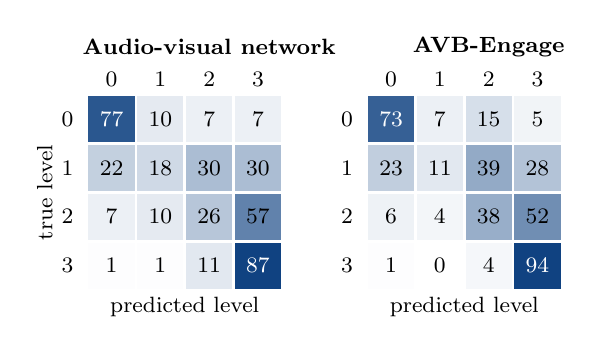
\begin{tikzpicture}[font=\footnotesize, cell/.style={minimum size=0.62cm, inner sep=0pt, draw=white, line width=1pt}]
\node[font=\footnotesize\bfseries] at (1.24,0.92) {Audio-visual network};
\node[anchor=east] at (-0.36,0.00) {0}; \node at (0.00,0.50) {0};
\node[cell, fill=seqhi!89!seqlo, text=white] at (0.00,0.00) {77};
\node[cell, fill=seqhi!11!seqlo] at (0.62,0.00) {10};
\node[cell, fill=seqhi!8!seqlo] at (1.24,0.00) {7};
\node[cell, fill=seqhi!8!seqlo] at (1.86,0.00) {7};
\node[anchor=east] at (-0.36,-0.62) {1}; \node at (0.62,0.50) {1};
\node[cell, fill=seqhi!25!seqlo] at (0.00,-0.62) {22};
\node[cell, fill=seqhi!20!seqlo] at (0.62,-0.62) {18};
\node[cell, fill=seqhi!35!seqlo] at (1.24,-0.62) {30};
\node[cell, fill=seqhi!35!seqlo] at (1.86,-0.62) {30};
\node[anchor=east] at (-0.36,-1.24) {2}; \node at (1.24,0.50) {2};
\node[cell, fill=seqhi!8!seqlo] at (0.00,-1.24) {7};
\node[cell, fill=seqhi!11!seqlo] at (0.62,-1.24) {10};
\node[cell, fill=seqhi!30!seqlo] at (1.24,-1.24) {26};
\node[cell, fill=seqhi!66!seqlo] at (1.86,-1.24) {57};
\node[anchor=east] at (-0.36,-1.86) {3}; \node at (1.86,0.50) {3};
\node[cell, fill=seqhi!1!seqlo] at (0.00,-1.86) {1};
\node[cell, fill=seqhi!1!seqlo] at (0.62,-1.86) {1};
\node[cell, fill=seqhi!12!seqlo] at (1.24,-1.86) {11};
\node[cell, fill=seqhi!100!seqlo, text=white] at (1.86,-1.86) {87};
\node at (0.93,-2.38) {predicted level};
\node[font=\footnotesize\bfseries] at (4.79,0.92) {AVB-Engage};
\node[anchor=east] at (3.19,0.00) {0}; \node at (3.55,0.50) {0};
\node[cell, fill=seqhi!84!seqlo, text=white] at (3.55,0.00) {73};
\node[cell, fill=seqhi!8!seqlo] at (4.17,0.00) {7};
\node[cell, fill=seqhi!17!seqlo] at (4.79,0.00) {15};
\node[cell, fill=seqhi!6!seqlo] at (5.41,0.00) {5};
\node[anchor=east] at (3.19,-0.62) {1}; \node at (4.17,0.50) {1};
\node[cell, fill=seqhi!26!seqlo] at (3.55,-0.62) {23};
\node[cell, fill=seqhi!12!seqlo] at (4.17,-0.62) {11};
\node[cell, fill=seqhi!45!seqlo] at (4.79,-0.62) {39};
\node[cell, fill=seqhi!32!seqlo] at (5.41,-0.62) {28};
\node[anchor=east] at (3.19,-1.24) {2}; \node at (4.79,0.50) {2};
\node[cell, fill=seqhi!7!seqlo] at (3.55,-1.24) {6};
\node[cell, fill=seqhi!5!seqlo] at (4.17,-1.24) {4};
\node[cell, fill=seqhi!43!seqlo] at (4.79,-1.24) {38};
\node[cell, fill=seqhi!60!seqlo] at (5.41,-1.24) {52};
\node[anchor=east] at (3.19,-1.86) {3}; \node at (5.41,0.50) {3};
\node[cell, fill=seqhi!1!seqlo] at (3.55,-1.86) {1};
\node[cell, fill=seqhi!0!seqlo] at (4.17,-1.86) {0};
\node[cell, fill=seqhi!4!seqlo] at (4.79,-1.86) {4};
\node[cell, fill=seqhi!100!seqlo, text=white] at (5.41,-1.86) {94};
\node at (4.48,-2.38) {predicted level};
\node[rotate=90] at (-0.85,-0.93) {true level};
\end{tikzpicture}

\end{document}
